\documentclass[border=5pt]{standalone}
\usepackage{tikz}
\usetikzlibrary{calc,fadings,decorations.pathreplacing,arrows,positioning}

\definecolor{arrowred}{RGB}{158, 125, 157}
\definecolor{gridyellow}{RGB}{234, 222, 255}

% The 3D code is based on The drawing is based on Tomas M. Trzeciak's 
% `Stereographic and cylindrical map projections example`: 
% http://www.texample.net/tikz/examples/map-projections/
\newcommand\pgfmathsinandcos[3]{%
	\pgfmathsetmacro#1{sin(#3)}%
	\pgfmathsetmacro#2{cos(#3)}%
}
\newcommand\LongitudePlane[3][current plane]{%
	\pgfmathsinandcos\sinEl\cosEl{#2} % elevation
	\pgfmathsinandcos\sint\cost{#3} % azimuth
	\tikzset{#1/.style={cm={\cost,\sint*\sinEl,0,\cosEl,(0,0)}}}
}
\newcommand\LatitudePlane[3][current plane]{%
	\pgfmathsinandcos\sinEl\cosEl{#2} % elevation
	\pgfmathsinandcos\sint\cost{#3} % latitude
	\pgfmathsetmacro\yshift{\cosEl*\sint}
	\tikzset{#1/.style={cm={\cost,0,0,\cost*\sinEl,(0,\yshift)}}} %
}
\newcommand\DrawLongitudeCircle[2][1]{
	\LongitudePlane{\angEl}{#2}
	\tikzset{current plane/.prefix style={scale=#1}}
	% angle of "visibility"
	\pgfmathsetmacro\angVis{atan(sin(#2)*cos(\angEl)/sin(\angEl))} %
	\draw[current plane,thin,black] (\angVis:1) arc (\angVis:\angVis+180:1);
	\draw[current plane,thin,dashed] (\angVis-180:1) arc (\angVis-180:\angVis:1);
}%this is fake: for drawing the grid
\newcommand\DrawLongitudeCirclered[2][1]{
	\LongitudePlane{\angEl}{#2}
	\tikzset{current plane/.prefix style={scale=#1}}
	% angle of "visibility"
	\pgfmathsetmacro\angVis{atan(sin(#2)*cos(\angEl)/sin(\angEl))} %
	\draw[current plane] (150:1) arc (150:180:1);
	%\draw[current plane,dashed] (-50:1) arc (-50:-35:1);
}%for drawing the grid
\newcommand\DLongredd[2][1]{
	\LongitudePlane{\angEl}{#2}
	\tikzset{current plane/.prefix style={scale=#1}}
	% angle of "visibility"
	\pgfmathsetmacro\angVis{atan(sin(#2)*cos(\angEl)/sin(\angEl))} %
	\draw[current plane,black,dashed, ultra thick] (150:1) arc (150:180:1);
}
\newcommand\DLatred[2][1]{
	\LatitudePlane{\angEl}{#2}
	\tikzset{current plane/.prefix style={scale=#1}}
	\pgfmathsetmacro\sinVis{sin(#2)/cos(#2)*sin(\angEl)/cos(\angEl)}
	% angle of "visibility"
	\pgfmathsetmacro\angVis{asin(min(1,max(\sinVis,-1)))}
	\draw[current plane,dashed,black,ultra thick] (-50:1) arc (-50:-35:1);
	
}
\newcommand\fillred[2][1]{
	\LongitudePlane{\angEl}{#2}
	\tikzset{current plane/.prefix style={scale=#1}}
	% angle of "visibility"
	\pgfmathsetmacro\angVis{atan(sin(#2)*cos(\angEl)/sin(\angEl))} %
	\draw[current plane,red,thin] (\angVis:1) arc (\angVis:\angVis+180:1);
	
}

\newcommand\DrawLatitudeCircle[2][1]{
	\LatitudePlane{\angEl}{#2}
	\tikzset{current plane/.prefix style={scale=#1}}
	\pgfmathsetmacro\sinVis{sin(#2)/cos(#2)*sin(\angEl)/cos(\angEl)}
	% angle of "visibility"
	\pgfmathsetmacro\angVis{asin(min(1,max(\sinVis,-1)))}
	\draw[current plane,thin,black] (\angVis:1) arc (\angVis:-\angVis-180:1);
	\draw[current plane,thin,dashed] (180-\angVis:1) arc (180-\angVis:\angVis:1);
}%Defining functions to draw limited latitude circles (for the red mesh)

\newcommand\DrawLatitudeCirclered[2][1]{
	\LatitudePlane{\angEl}{#2}
	\tikzset{current plane/.prefix style={scale=#1}}
	\pgfmathsetmacro\sinVis{sin(#2)/cos(#2)*sin(\angEl)/cos(\angEl)}
	% angle of "visibility"
	\pgfmathsetmacro\angVis{asin(min(1,max(\sinVis,-1)))}
	%\draw[current plane,red,thick] (-\angVis-50:1) arc (-\angVis-50:-\angVis-20:1);
	\draw[current plane] (-50:1) arc (-50:-35:1);
}


\newcommand\DrawLatitudeCircleredCoord[4][1]{
	\LatitudePlane{\angEl}{#2}
	\tikzset{current plane/.prefix style={scale=#1}}
	\pgfmathsetmacro\sinVis{sin(#2)/cos(#2)*sin(\angEl)/cos(\angEl)}
	% angle of "visibility"
	\pgfmathsetmacro\angVis{asin(min(1,max(\sinVis,-1)))}
	%\draw[current plane,red,thick] (-\angVis-50:1) arc (-\angVis-50:-\angVis-20:1);
	\draw[current plane] (-50:1) coordinate (#3) arc (-50:-35:1) coordinate (#4);
}

\newcommand\DrawLongitudeCircleredCoord[4][1]{
	\LongitudePlane{\angEl}{#2}
	\tikzset{current plane/.prefix style={scale=#1}}
	% angle of "visibility"
	\pgfmathsetmacro\angVis{atan(sin(#2)*cos(\angEl)/sin(\angEl))} %
	\draw[current plane] (150:1) coordinate (#3) arc (150:180:1) coordinate (#4);
	%\draw[current plane,dashed] (-50:1) arc (-50:-35:1);
}%for drawing the grid

\tikzset{%
	>=latex,
	inner sep=0pt,%
	outer sep=2pt,%
	mark coordinate/.style={inner sep=0pt,outer sep=0pt,minimum size=3pt,
		fill=black,circle}%
}

\definecolor{myblue}{RGB}{158, 156, 219} 
\definecolor{myred}{RGB}{234, 222, 255}
\definecolor{myorange}{RGB}{255, 102, 0}

\begin{document}
	
	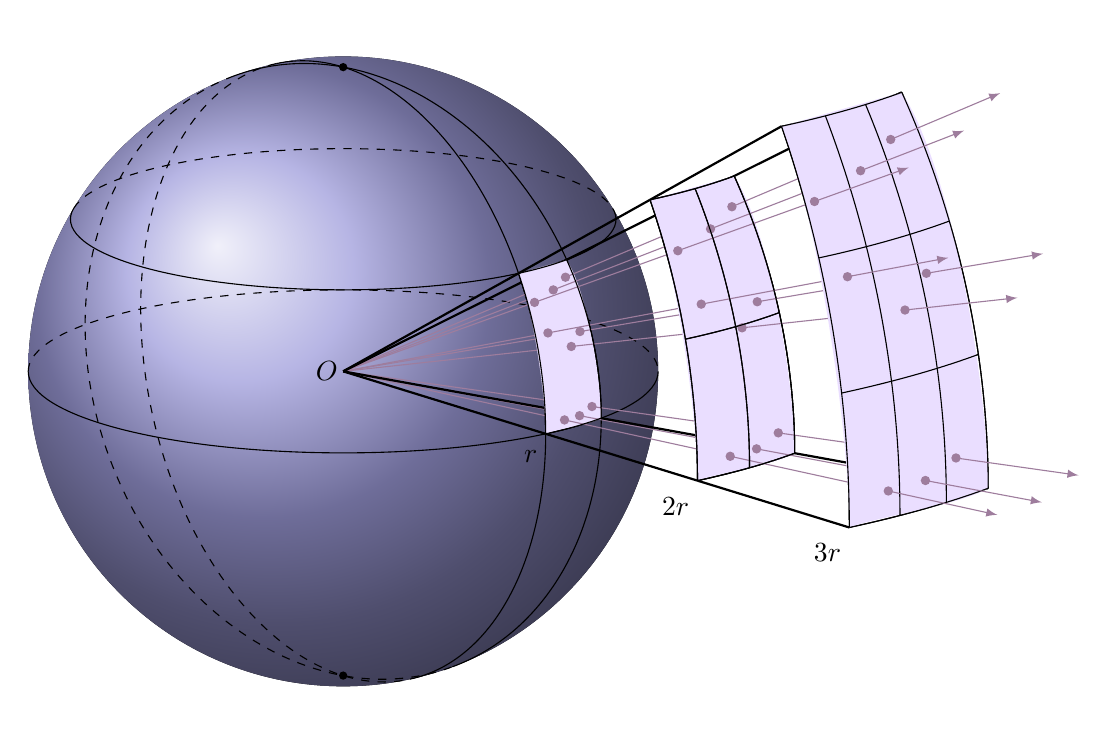
\begin{tikzpicture}[scale=1,node/.style={minimum size=1cm}]
		\def\R{4} % sphere radius
		\def\angEl{15} % elevation angle
		\def\angAz{-100} % azimuth angle
		\def\angPhiOne{-50} % longitude of point P
		\def\angPhiTwo{-35} % longitude of point Q
		\def\angBeta{30} % latitude of point P and Q
		
		%% working planes
		\pgfmathsetmacro\H{\R*cos(\angEl)} % distance to north pole
		
		%drawing the sphere
		\fill[ball color=myblue] (0,0) circle (\R);
		\coordinate (O) at (0,0);
		\coordinate[mark coordinate] (N) at (0,\H);
		\coordinate[mark coordinate] (S) at (0,-\H);
		
		\DrawLongitudeCircle[\R]{\angPhiOne} % pzplane
		\DrawLongitudeCircle[\R]{\angPhiTwo} % qzplane
		\DrawLatitudeCircle[\R]{\angBeta}
		\DrawLatitudeCircle[\R]{0} % equator
		
		%drawing the outermost grid and
		%locating some special points in its border
		\DrawLongitudeCircleredCoord[\R+6]{130}{11}{41}
		\DrawLongitudeCircleredCoord[\R+6]{135}{12}{42}
		\DrawLongitudeCircleredCoord[\R+6]{140}{13}{43}
		\DrawLongitudeCircleredCoord[\R+6]{145}{14}{44}
		
		\DrawLatitudeCircleredCoord[\R+6]{0}{41}{44}
		\DrawLatitudeCircleredCoord[\R+6]{10}{31}{34}
		\DrawLatitudeCircleredCoord[\R+6]{20}{21}{24}
		\DrawLatitudeCircleredCoord[\R+6]{30}{11}{14}
		
		%drawing the middle grid and
		%locating some special points in its border
		\DrawLongitudeCircleredCoord[\R+3]{130}{m11}{m31}
		\DrawLongitudeCircleredCoord[\R+3]{137.5}{m12}{m32}
		\DrawLongitudeCircleredCoord[\R+3]{145}{m13}{m33}
		
		\DrawLatitudeCircleredCoord[\R+3]{0}{m31}{m34}
		\DrawLatitudeCircleredCoord[\R+3]{15}{m21}{m24}
		\DrawLatitudeCircleredCoord[\R+3]{30}{m11}{m14}
		
		%drawing the grid on the sphere and
		%locating some special points in its border
		\DrawLongitudeCircleredCoord[\R]{130}{i11}{i21}
		\DrawLongitudeCircleredCoord[\R]{145}{i12}{i22}
		
		\DrawLatitudeCircleredCoord[\R]{0}{i21}{i22}
		\DrawLatitudeCircleredCoord[\R]{30}{i11}{i12}
		
		
		%locating coordinates for the arrows from the origin
		\coordinate (P1) at  ( $ (11)!0.2!(43) $ ); 
		\coordinate (P2) at  ( $ (13)!0.3!(24) $ );
		\coordinate (P3) at  ( $ (12)!0.23!(34) $ );
		
		\coordinate (P4) at  ( $ (11)!0.4!(43) $ );
		\coordinate (P5) at  ( $ (21)!0.54!(34) $ );
		\coordinate (P6) at  ( $ (12)!0.66!(34) $ );
		
		\coordinate (P7) at  ( $ (31)!0.8!(42) $ ); 
		\coordinate (P8) at  ( $ (31)!0.8!(43) $ ); 
		\coordinate (P9) at  ( $ (34)!0.7!(43) $ ); 
		
		
		%locating the coordinates for the dots on the grids
		\foreach \Valor in {1,2,3,4,5,6,7,8,9} 
		{
			\path[] (O) -- (P\Valor)
			coordinate[pos=1] (punto-out-\Valor) {}
			coordinate[pos=0.71] (punto-middle-\Valor) {}
			coordinate[pos=0.406] (punto-on-\Valor) {};
		}
		
		% draw arrows from the origin to the grid on the sphere
		\foreach \Valor in {1,...,9}
		{
			\draw[arrowred] (O) -- (punto-on-\Valor);
		}
		
		%drawing the frames from the origin to the grid on the sphere
		\foreach \Valor in {11,12,21,22}
		{
			\draw[thick] (O) -- (i\Valor);
		}
		
		% filling the grid on the sphere
		% and redrawing it
		\fill[gridyellow]
		(i11) -- 
		(i12) to[out=-57,in=90,looseness=0.6] 
		(i22) to[out=-150,in=20,looseness=0.6] 
		(i21) to[out=90,in=-68,looseness=0.6] 
		(i11);
		
		%placing the dots on the grid on the sphere
		\foreach \Valor in {1,2,3,4,5,6,7,8,9} 
		{
			\node[fill,circle,fill=arrowred,inner sep=1.2pt] at (punto-on-\Valor) {};
		}
		
		% draw arrows from the grid on the sphere to the middle grid
		\foreach \Valor in {1,...,9}
		{
			\draw[arrowred] (punto-on-\Valor) -- (punto-middle-\Valor);
		}
		
		%drawing the frames from the grid on the sphere
		% to the middle grid
		\foreach \iValor/\fValor in {11/11,12/13,21/31,22/33}
		{
			\draw[thick] (i\iValor) -- (m\fValor);
		}
		
		% filling the middle grid
		% and redrawing it
		\fill[gridyellow]
		(m11) -- 
		(m13) to[out=-57,in=90,looseness=0.6] 
		(m33) to[out=-150,in=20,looseness=0.6] 
		(m31) to[out=90,in=-68,looseness=0.6] 
		(m11);
		\DrawLongitudeCircleredCoord[\R+3]{130}{m11}{m31}
		\DrawLongitudeCircleredCoord[\R+3]{137.5}{m12}{m32}
		\DrawLongitudeCircleredCoord[\R+3]{145}{m13}{m33}
		
		\DrawLatitudeCircleredCoord[\R+3]{0}{m31}{m34}
		\DrawLatitudeCircleredCoord[\R+3]{15}{m21}{m24}
		\DrawLatitudeCircleredCoord[\R+3]{30}{m11}{m14}
		
		%placing the dots on the middle grid
		\foreach \Valor in {1,2,3,4,5,6,7,8,9} 
		{
			\node[fill,circle,fill=arrowred,inner sep=1.2pt] at (punto-middle-\Valor) {};
		}
		
		% draw arrows from the middle grid to the outermost grid
		\foreach \Valor in {1,...,9}
		{
			\draw[arrowred] (punto-middle-\Valor) -- (punto-out-\Valor);
		}
		
		%drawing the frames from the middle grid 
		% to the outermost grid
		\foreach \iValor/\fValor in {11/11,13/14,31/41,33/44}
		{
			\draw[thick] (m\iValor) -- (\fValor);
		}
		
		% filling the outermost grid
		% and redrawing it
		\fill[gridyellow]
		(11) -- 
		(14) to[out=-57,in=90,looseness=0.6] 
		(44) to[out=-150,in=20,looseness=0.6] 
		(41) to[out=90,in=-68,looseness=0.6] 
		(11);
		\DrawLongitudeCircleredCoord[\R+6]{130}{11}{41}
		\DrawLongitudeCircleredCoord[\R+6]{135}{12}{42}
		\DrawLongitudeCircleredCoord[\R+6]{140}{13}{43}
		\DrawLongitudeCircleredCoord[\R+6]{145}{14}{44}
		
		\DrawLatitudeCircleredCoord[\R+6]{0}{41}{44}
		\DrawLatitudeCircleredCoord[\R+6]{10}{31}{34}
		\DrawLatitudeCircleredCoord[\R+6]{20}{21}{24}
		\DrawLatitudeCircleredCoord[\R+6]{30}{11}{14}
		
		%placing the dots on the outermost grid
		\foreach \Valor in {1,2,3,4,5,6,7,8,9} 
		{
			\node[fill,circle,fill=arrowred,inner sep=1.2pt] at (punto-out-\Valor) {};
		}
		
		%drawing arrows from the outermost grid
		\foreach \Valor in {1,2,3,4,5,6,7,8,9} 
		{
			\coordinate (end-arrow-\Valor) at ( $ (O)!1.2!(P\Valor) $ );
		}  
		
		%drawing arrows from the outermost grid
		\foreach \Valor in {1,2,3,4,5,6,7,8,9} 
		{
			\draw[arrowred,-latex] (punto-out-\Valor) -- (end-arrow-\Valor);
		}  
		
		
		%drawing grid on the spere
		\foreach \t in {130,145} { \DrawLongitudeCirclered[\R]{\t} }
		\foreach \t in {0,30} { \DrawLatitudeCirclered[\R]{\t} }
		
		%drawing the middle grid
		\foreach \t in {130,137.5,145} { \DrawLongitudeCirclered[\R+3]{\t} }
		\foreach \t in {0,15,30} { \DrawLatitudeCirclered[\R+3]{\t} }
		
		%labels
		\node[left] at (O) {$O$};
		\node[below left=4pt and 1pt] at (i21) {$r$};
		\node[below left=4pt and 1pt] at (m31) {$2r$};
		\node[below left=4pt and 1pt] at (41) {$3r$};
	\end{tikzpicture}
	
\end{document} 